\section{Hagan Rowlenstino/1174040}
	\subsection{Soal 1}
	library matplotlib adalah sebuah library untuk memplotting 2 Dimensi yang output nya adalah gambar publikasi yang bermutu di banyak format hardocpy serta lingkungan interaktif berbagai platform

	\subsection{Soal 2}
	untuk membuat sumbu x dan y :
	\lstinputlisting{src/6/1174040/Teori/chap6_1174040_2.py}

	\subsection{Soal 3}
	\begin{itemize}
		\item PLot Garis :

		\lstinputlisting[firstline=8, lastline=13]{src/6/1174040/Teori/chap6_1174040_3.py}

		\item Plot Sebaran

		\lstinputlisting[firstline=15, lastline=18]{src/6/1174040/Teori/chap6_1174040_3.py}

		\item Plot Batang / Histogram

		\lstinputlisting[firstline=20, lastline=23]{src/6/1174040/Teori/chap6_1174040_3.py}

		\item Pie

		\lstinputlisting[firstline=26, lastline=35]{src/6/1174040/Teori/chap6_1174040_3.py}

	\end{itemize}

	\subsection{Soal 4}
	\begin{itemize}
		\item Legend : Penjelasan garis beserta contoh dari garis yang dijelaskan tersebut. untuk membuat legend dapat menggunakan sintaks berikut :

		\begin{verbatim} legend('legend grafik1',…,'legend grafikN','Nilai Pos') \end{verbatim}
		
		\item Label : Memberikan penamaan untuk skala(sumbu) yang kita buat. untuk menambahkan label, kita dapat menggunakan sintaks berikut :

		\begin{verbatim} 
		xlabel(‘teks horizontal axis’)

		ylabel(‘teks vertikal axis’)
		\end{verbatim}
	\end{itemize}

	\subsection {Soal 5}
	Subplot pada matplotlib berfungsi untuk membuat banyak plot grafik dalam satu figure saja.
	dimana  subplot dapat kita definisikan sebagai berikut :
	
	\begin{verbatim} subplot(m,n,i) 
	\end{verbatim}
	Dimana m adalah tinggi nya, n adalah lebar nya dan i adalah urutan penempatannya.
	Untuk membuat 9 subplot dapat dilihati dari contoh dibawah ini :

	\lstinputlisting{src/6/1174040/Teori/chap6_1174040_5.py}

	\begin{figure}[ht]
            \centerline{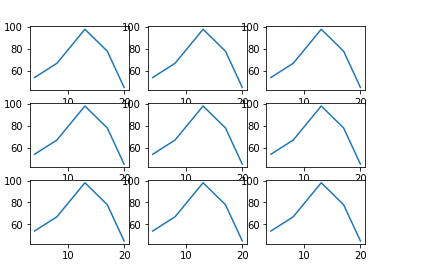
\includegraphics[width=0.5\textwidth]{figures/6/1174040/Teori/1174040_no5.png}}
            \caption{No. 5}
            \label{1174040_chap6_no5}
            \end{figure}

	\subsection{Soal 6}
	color yang dapat digunakan adalah red(r),blue(b),green(g),cyan(c),magenta(m),yellow(y),black(k),white(w)

	\subsection{Soal 7}
	fungsi Hist digunakan untuk membuat histogram yang berfungsi untuk menampilkan frekuensi data dengan menggunakan grafik batang

	\lstinputlisting{src/6/1174040/Teori/chap6_1174040_hist.py}

	\begin{figure}[ht]
            \centerline{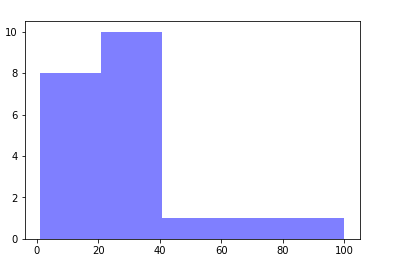
\includegraphics[width=0.5\textwidth]{figures/6/1174040/Teori/1174040_no7.png}}
            \caption{No. 7}
            \label{1174040_chap6_no7}
            \end{figure}

	\subsection{Soal 8}
	\begin{itemize}
		\item Labels : Untuk memberi penamaan terhadap setiap potongan dari pie
		\item colors : Untuk memberikan warna spesifik terhadap potongan potongan pie, jika tidak diberi warna maka dia akan menggambi warna dari pie yang telah berjalan
		\item startangle : Untuk menetapkan dari sudut mana grafik tersebut akan dimulai
		\item shadow : untuk memberikan efek bayangan di bawah pie maupun potongannya
		\item explode : untuk menentukan seerapa jauh pemisahkan potongan pie dari potongan - potongan lainnya
		\item autopct : untuk memberikan nilai atau skalal numeric pada label didalam potongan pie . seperti mengubah dari 10 menjadi 10.0
	\end{itemize}

	\subsection{Cek Plagiarisme}
	
	\begin{figure}[ht]
            \centerline{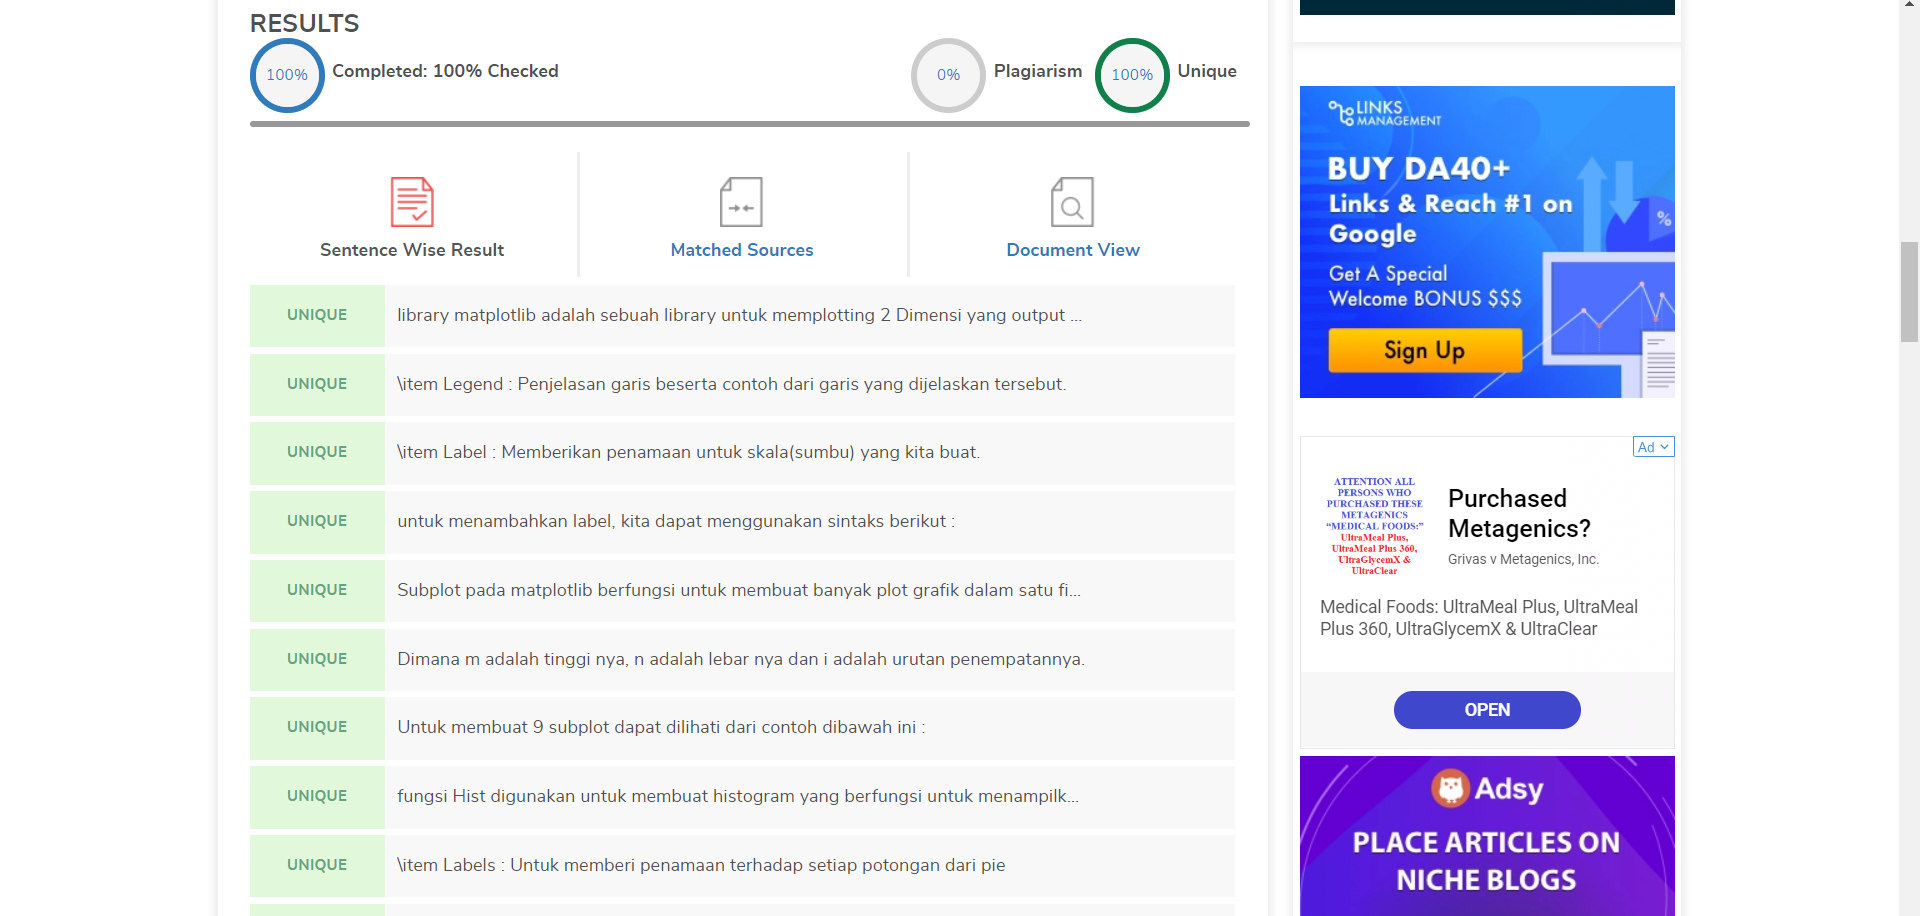
\includegraphics[width=0.5\textwidth]{figures/6/1174040/Teori/1174040_plagiat.png}}
            \caption{Cek Plagiarisme}
            \label{1174040_chap6_plagiat}
            \end{figure}